\documentclass[times,specification,annotation]{itmo-student-thesis}

%% Опции пакета:
%% - specification - если есть, генерируется задание, иначе не генерируется
%% - annotation - если есть, генерируется аннотация, иначе не генерируется
%% - times - делает все шрифтом Times New Roman, собирается с помощью xelatex
%% - pscyr - делает все шрифтом Times New Roman, требует пакета pscyr.

%% Делает запятую в формулах более интеллектуальной, например:
%% $1,5x$ будет читаться как полтора икса, а не один запятая пять иксов.
%% Однако если написать $1, 5x$, то все будет как прежде.
\usepackage{icomma}

%% Один из пакетов, позволяющий делать таблицы на всю ширину текста.
\usepackage{tabularx}

%% Данные пакеты необязательны к использованию в бакалаврских/магистерских
%% Они нужны для иллюстративных целей
%% Начало
\usepackage{tikz}
\usetikzlibrary{arrows,automata,positioning}
\usepackage{filecontents}
\begin{filecontents}{bachelor-thesis.bib}
@article { state-merging-dfa,
    author      = {Bernard Lambeau and Christophe Damas and Pierre Dupont},
    title       = {State-Merging DFA Induction Algorightms with Mandatory Merge Constraints},
    pages       = {139-153},
    journal     = {Lecture Notes in Computer Science},
    year        = {2008},
    langid      = {english},
    url         = {https://www.info.ucl.ac.be/~pdupont/pdupont/pdf/icgi08.pdf}
}

@article { 1-dta
    author      = {Sicco Verwer and Mathijs de Weerdt and Cees Witteveen},
    title       = {The efficiency of identifying timed automata and the power of clocks},
    pages       = {606-625},
    journal     = {Information and Computation},
    year        = {2011},
    langid      = {english},
    url         = {http://wwwis.win.tue.nl/~sverwer}
}

@article { rti,
    author      = {Sicco Verwer and Mathijs de Weerdt and Cees Witteveen},
    title       = {Efficiently identifying deterministic real-time automatafrom labeled data},
    pages       = {295-333},
    journal     = {Springer},
    year        = {2010},
    langid      = {english},
    url         = {https://link.springer.com/article/10.1007/s10994-011-5265-4}
}

@article { timed-k-tail,
    author      = {Fabrizio Pastore and Daniela Micucci and Leonardo Mariani},
    title       = {Timed k-Tail: Automatic Inference of Timed Automata},
    numpages    = {11},
    pagetotal   = {11},
    year        = {2017},
    langid      = {english},
    url         = {https://arxiv.org/pdf/1705.08399.pdf}
}

@article { k-tail,
    author      = {Alan Biermann and Jerome Feldman},
    title       = {On the Synthesis of Finite-State Machines from Samples of Their Behavior},
    pages       = {592-597},
    journal     = {IEEE Transactions on Computers},
    year        = {1972},
    langid      = {english},
    url         = {https://www.researchgate.net/publication/224483188_On_the_Synthesis_of_Finite-State_Machines_from_Samples_of_Their_Behavior}
}

@article { rti-plus,
    author      = {Sicco Verwer},
    title       = {Efficient identification of timed automata: Theory and practice},
    numpages    = {252},
    pagetotal   = {252},
    year        = {2010},
    langid      = {english},
    url         = {https://www.narcis.nl/publication/RecordID/oai:tudelft.nl:uuid:61d9f199-7b01-45be-a6ed-04498113a212}
}

@article { moha,
    author      = {Qin Lin and Yihuan Zhang and Sicco Verwer and Jun Wang},
    title       = {MOHA: a Multi-mode Hybrid Automaton Model for Learning Car-following Behaviors},
    pages       = {790-796},
    year        = {2018},
    langid      = {english},
    url         = {https://ieeexplore.ieee.org/document/8384014}
}

@article { bfs,
    author      = {Ilya Zakirzyanov and Anatoly Shalyto and Vladimir Ulyantsev},
    title       = {Finding all minimum-size DFA consistent withgiven examples: SAT-based approach},
    numpages    = {15},
    pagetotal   = {15},
    year        = {2017},
    langid      = {english},
    url         = {http://pages.di.unipi.it/datamod/wp-content/uploads/sites/8/2017/08/Zakirzyanov-Shalyto-Ulyantsev_DataMod2017.pdf}
}
\end{filecontents}
%% Конец

%% Указываем файл с библиографией.
\addbibresource{bachelor-thesis.bib}

\begin{document}

\studygroup{M3439}
\title{Пример оформления ВКР бакалавра}
\author{Костливцев Никита Алексеевич}{Костливцев Н.А.}
\supervisor{Чивилихин Даниил Сергеевич}{Чивилихин Д.С.}{к.т.н.}{научный сотрудник Университета ИТМО}
\publishyear{2019}
%% Дата выдачи задания. Можно не указывать, тогда надо будет заполнить от руки.
\startdate{01}{сентября}{2018}
%% Срок сдачи студентом работы. Можно не указывать, тогда надо будет заполнить от руки.
\finishdate{31}{мая}{2019}
%% Дата защиты. Можно не указывать, тогда надо будет заполнить от руки.
\defencedate{19}{июня}{2019}

???\addconsultant{Белашенков Н.Р.}{канд. физ.-мат. наук, без звания}

\secretary{Павлова О.Н.}

%% Задание
%%% Техническое задание и исходные данные к работе
\technicalspec{???Чем отличается от следующего???}

%%% Содержание выпускной квалификационной работы (перечень подлежащих разработке вопросов)
\plannedcontents{
\begin{enumerate}
  \item Постановка задачи и исследование существующих на данный момент решений
  \item Описание разработанных идей и их программная реализация
  \item Тестирование реализованных идей, сравнение с существующими подходами
\end{enumerate}
}

%%% Исходные материалы и пособия 
\plannedsources{Опубликованные статьи на тему ``Синтез временных автоматов'' и статей, демонстрирующих использование временных автоматов}

%%% Цель исследования
\researchaim{ Разработка методов синтеза временных автоматов на основе программирования в ограничениях }

%%% Задачи, решаемые в ВКР
\researchtargets{Что написать???}

???%%% Использование современных пакетов компьютерных программ и технологий
\addadvancedsoftware{Пакет \texttt{tabularx} для чуть более продвинутых таблиц}{\ref{sec:tables}, Приложения~\ref{sec:app:1}, \ref{sec:app:2}}
\addadvancedsoftware{Пакет \texttt{biblatex} и программное средство \texttt{biber}}{Список использованных источников}

%%% Краткая характеристика полученных результатов 
\researchsummary{Удалось получить работоспособный алгоритм, способный синтезировать временные автоматы}

%%% Гранты, полученные при выполнении работы 
\researchfunding{Автор разрабатывал этот алгоритм исключительно за свой счет и на
добровольных началах при огромной помощи своего научного руководителя.}

%%% Наличие публикаций и выступлений на конференциях по теме выпускной работы
\researchpublications{По теме этой работы публикаций не было.}

%% Эта команда генерирует титульный лист и аннотацию.
\maketitle{Бакалавр}

%% Оглавление
\tableofcontents

%% Макрос для введения. Совместим со старым стилевиком.
\startprefacepage

Существует множество систем реального времени, поведение которых существенно зависит от времени. Поведение данных систем часто не поддается описанию вручную. Поэтому его
моделируют с помощью вычилительных устройств, исходя из примеров поведения. На текущий момент лучшей моделью для описания данного вида систем является временной автомат.
Следуя принципу бритвы Окамма, лучшей сгенерированной моделью, описывающей систему, будет являться модель, использующая наименьшее число сущностей, как следствие,
наилучшим автоматом, описывающим систему реального времени, будет являться минимальный. Существующие на текущий момент state-of-the-art решения генерируют приблизительно минимальный
автомат. Новый предоставленный алгоритм генерирует минимальный автомат в обязательном порядке. Но остро стоит вопрос о разумности использования такого решения из-за
возможно медленной скорости работы. Также временные автоматы последнее время используются в машинном обучении, о чем свидетельствует статья~\cite{moha}, поэтому на сегодняшний день
разработка новых методов генерации временных автоматов является актуальной задачей. 

В главе 1 описаны основные термины, приведены основные результаты и методы синтеза детерминированных временных автоматов.

В главе 2 приведен новый метод синтеза детерминированных временных автоматов.

В главе 3 было проведено тестирование нового метода и его сравнение с существующими решениями.

%% Начало содержательной части.
\chapter{Временные автоматы, методы их синтеза}

\section{Термины и понятия}
В данном разделе будут приведены определения терминов, которые будут использоваться в следующих главах, а также основные результаты о временных автоматах.

\begin{definition}
  Временное ограничение $g$ -- предикат на таймерах. Его можно получить одним из трех способов:
  \begin{itemize}
    \item $g := c \leq x$
    \item $g := c \geq x$
    \item $g := g_1 \land g_2$
  \end{itemize}
  где $g$ -- временное ограничение, $c \in C$ -- таймер, $x \in \mathbb{N}$ -- граница ограничения
\end{definition}

\begin{definition}
  Временной автомат $\mathcal{A}$ -- кортеж $\langle \Sigma, Q, q_0, C, \Delta, F \rangle$, где
  \begin{itemize}
    \item $\Sigma$ -- алфавит(множество символов) автомата,
    \item $Q$ -- конечное множество состояний,
    \item $q_0 \in Q$ -- начальное состояние автомата,
    \item $C$ -- конечное множество таймеров,
    \item $F \subseteq Q$ -- множество принимающих состояний.
    \item $\Delta$ -- конечное множество переходов, где переход -- это кортеж $\langle q_1, q_2, a, g, R \rangle$, где
    \begin{itemize}
      \item $q_1, q_2 \in Q$ -- начальное и конечное состояние, которые соединяет данный переход,
      \item $a \in \Sigma$ -- символ, по которому осуществляется переход,
      \item $g$ -- временные ограничения на таймерах,
      \item $R \in 2^{C}$ -- таймеры, которые нужно сбросить после перехода по $\delta$. 
    \end{itemize}
  \end{itemize}
  \label{timed-automaton}
\end{definition}

\begin{example}
  На рисунке~\ref{time_automaton} приведен пример временного автомата. 
  Состояние $q_3$ является принимающим, все же остальные принимающими не являются. 
  Начальным состоянием временного автомата является $q_0$. 
  Из него исходит одно ребро в состояние $q_1$ с символом перехода $a$. 
  После перехода по данному ребру таймер $x$ сбрасывается. 
  Из состояния $q_1$ тоже исходит ребро в состояние $q_2$ с символом перехода $b$, но уже с ограничением на таймер $x$.
  Чтобы пройти по данному ребру таймер $x$ должен быть меньше единицы.
  Лучше всего использование таймеров демонстрируют два перехода из состояния $q_2$, так как из-за таймеров, 
  чтобы пройти в состояние $q_3$, необходимо будет 20 раз пройти по петле в то же состояние $q_2$.
\end{example}

\begin{figure}[!h]
\caption{Пример временного автомата}\label{time_automaton}
\centering
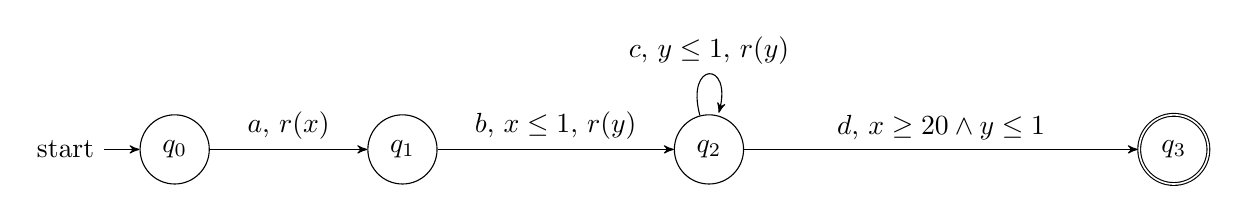
\begin{tikzpicture}[>=stealth']
  \node[state, initial] (q0) {$q_0$};
  \node[state] (q1) [right=2cm of q0] {$q_1$};
  \node[state] (q2) [right=3cm of q1] {$q_2$};
  \node[state, accepting] (q3) [right=5cm of q2] {$q_3$};
  \path[->]
  (q0) edge node[anchor=center, above] {$a$, $r(x)$} (q1)
  (q1) edge node[anchor=center, above] {$b$, $x \leq 1$, $r(y)$} (q2)
  (q2) edge [loop above] node[anchor=center, above] {$c$, $y \leq 1$, $r(y)$} ()
       edge node[anchor=center, above] {$d$, $x \geq 20 \land y \leq 1$} (q3);
\end{tikzpicture}
\end{figure}

\begin{definition}
  Трассировка $\tau$ -- последовательность пар $\{\left( a, t \right)\}$, 
  где $t \in \mathbb{N}$ -- задержка между предыдущим и текущим событиями, $a \in \Sigma$ -- символ перехода.
\end{definition}

\begin{definition}
  Значение $\nu(x)$ таймера $x \in C$ -- функция из таймера $x$ в $\mathbb{N}$
\end{definition}

\begin{definition}
  Путь во временном автомате по трассировке $\{\left( a_i, d_i \right)\}$ -- последовательность из пар $\{\left( q_i, \nu_i \right)\}$ таких, 
  что $q_i \in Q$ -- состояние на шаге $i$, $\nu_i$ -- значения таймеров на шаге $i$ и для которых выполняются следующие ограничения:
  \begin{itemize}
    \item $q_{2i} = q_{2i+1}$
    \item $\forall x \in C: \nu_{2i+1}(x) - \nu_{2i}(x) = d_i$
    \item $\exists! \langle q^1, q^2, a, g, R \rangle \in \Delta$: 
      \begin{itemize}
	\item $q_{2i+1} = q^1$
	\item $q_{2i+2} = q^2$
        \item $\forall x \in R: \nu_{2i+2}(x) = 0$
	\item $\forall x \not\in R: \nu_{2i+2}(x) = \nu_{2i+1}(x)$
	\item $\forall x \in C: \nu_{2i+1}(x)$ удовлетворяет $g$
      \end{itemize}
  \end{itemize}
\end{definition}

Другими словами, в пути во временном автомате каждая пара из состояния и значений таймеров с 
четным номером отличается от предыдущей изменением состояния автомата, а также, возможно, сбрасыванием некоторого количества таймеров, 
каждая же пара с нечетным индексом отличается от предыдущей только увеличением значений таймеров.

\begin{definition}
  Детерминированный временной автомат $\mathcal{A}$ -- временной автомат, для которого не существует трассировки, для которой существует два корректных пути в данном временном автомате.
  \label{DTA}
\end{definition}

В дальнейшем, если это не оговорено заранее, под понятием временного автомата будет подразумеваться детерминированный временной автомат.

\begin{definition}
  Языком $\mathcal{L}(\mathcal{A})$ временного автомата $\mathcal{A}$ назовем множество всех принимаемых трассировок.
\end{definition}

\begin{definition}
  Класс автоматов $\mathbb{K}$ называется достижимым за полином, если существует полином $p$ такой, что для любых
  $\mathcal{A} \in \mathbb{K}, q \in Q_{\mathcal{A}}$ существует трассировка $\tau$ такая, что порожденный ей путь заканчивается в $q$ и $|\tau| < p(|\mathcal{A}|)$.
\end{definition}

Приведем так же определения более слабого класса временных автоматов -- автоматов реального времени.

\begin{definition}
  Автомат реального времени -- временной автомат такой, что $C = \{c_0\}, R_{\delta} = \{c_0\}$ для любого перехода $\delta \in \Delta$.
  \label{rti}
\end{definition}

\begin{definition}
  Вероятностный детерминированный автомат реального времени -- кортеж $\langle \mathcal{A}, \mathcal{E}, \mathcal{T}, \mathcal{H} \rangle$, где
  \begin{itemize}
    \item $\mathcal{A} = \langle \Sigma, Q, q_0, C, \Delta, F \rangle$ -- автомат реального времени,
    \item $\mathcal{E}: Q \times \Sigma \rightarrow [0, 1]$ -- распределение вероятностей на множестве символов перехода,
    \item $\mathcal{T}: Q \times \mathcal{H} \rightarrow [0, 1]$ -- распределение вероятностей на множестве времен ожидания для данного интервала $h \in \mathcal{H}$,
    \item $\mathcal{H}$ -- конечное множество неперекрывающихся интервалов.
  \end{itemize}
  \label{rti++}
\end{definition}

\section{Известные результаты}
Следующие результаты были получены авторами статьи~\cite{1-dta}.

\begin{lemma}
  Класс временных автоматов не является достижимым за полином.
  \label{unreachable_lemma}
\end{lemma}

Лемма~\ref{unreachable_lemma} фактически утверждает, что, чтобы однозначно правильно синтезировать 
автомат по примерам, необходимо в качество примеров иметь так же пример экспоненциальной длины от размера временного автомата.

\begin{definition}
  Класс автоматов $\mathbb{K}$ называется различимым за полином, если существует полином $p$ такой, что для любых
  $\mathcal{A}, \mathcal{A'} \in \mathbb{K}, \mathcal{L}(\mathcal{A}) \neq \mathcal{L}(\mathcal{A'})$ существует трассировка $\tau$ такая, что 
  $\tau \in \mathcal{L}(\mathcal{A}) \Delta \mathcal{L}(\mathcal{A'})$ и $|\tau| < p(|\mathcal{A}| + |\mathcal{A'}|)$
\end{definition}

\begin{lemma}
  Класс временных автоматов не различим за полином.
  \label{distinguishability_lemma}
\end{lemma}

\begin{definition}
    Характеристическим множеством языка $\mathcal{L}_t$ для алгоритма $A$ называется множество трассировок $S_{cs} = \{S_{cs+}, S_{cs-}\}$, где
  $S_{cs+} \subseteq \mathcal{L}_t$, $S_{cs-} \subseteq \mathcal{L}_t^c$, такое, что 
  для любого $S \supseteq S_{cs}, S_+ \subseteq \mathcal{L}_t, S_- \subseteq \mathcal{L}_t^c$ алгоритм $A$ на вход $S$ вернет автомат $\mathcal{A}$ такой, что $\mathcal{L}(\mathcal{A}) = \mathcal{L}_t$.
\end{definition}

\begin{definition}
    Класс автоматов $\mathbb{K}$ является эффективно синтезируемым в пределе, если существуют полиномы $p, q$ и алгоритм $A$ такие, что
  \begin{itemize}
    \item Время работы алгоритма на входе $S$ ограничено сверху $p(\mathop{\sum}\limits_{\tau \in S}|\tau|)$
    \item Для любого языка $\mathcal{A} \in \mathbb{K}$ существует $S_{cs} $ 
      -- характеристическое множество языка $\mathcal{A}$ для алгоритма $A$ такой, что $\mathop{\sum}\limits_{\tau \in S_{cs}}|\tau| < q(|\mathcal{A}|)$
  \end{itemize}
\end{definition}

\begin{theorem}
    Класс временных автоматов не является эффективно синтезируемым
  \label{efficient_synthesis_theorem}
\end{theorem}

Доказаны также более сильные варианты данной теоремы.

\begin{theorem}
  Если $coNP \neq PSPACE$, то временной автомат не может быть эффективно синтезирован.
  \label{coNPneqPSPACE_lemma}
\end{theorem}

\begin{theorem}
  Если $NP \neq PSPACE$, то временной автомат не может быть эффективно синтезирован.
  \label{NPneqPSPACE_lemma}
\end{theorem}

Хоть и было доказано, что класс временных автоматов в целом не является эффективно синтезируемым, из него возможно выделить подкласс временных автоматов, 
который бы являлся эффективно синтезируемым. Приведем формулировку теоремы, которая немного проясняет ситуацию с временными автоматами.

\begin{theorem}
  Класс временных автоматов, в котором используется два или больше таймеров не может быть эффективно синтезирован.
  \label{two_or_more_timers_lemma}
\end{theorem}

Таким образом, возможно стоит обратить внимание на подкласс временных автоматов, которые могут использовать всего один таймер? 
На самом деле в статье~\cite{1-dta} были также доказаны следующие факты:

\begin{lemma}
  Класс временных автоматов с одним таймером является полиномиально достижимым.
  \label{reachability_1_lemma}
\end{lemma}

\begin{lemma}
  Класс временных автоматов с одним таймером является полиномиально различимым.
  \label{distinguishability_1_lemma}
\end{lemma}

\begin{theorem}
  Класс временных автоматов с одним таймером является эффективно синтезируемым.
  \label{efficient_synthesis_1_theorem}
\end{theorem}

В качестве доказательства теоремы~\ref{efficient_synthesis_1_theorem} авторы статьи~\cite{1-dta} предоставили алгоритм ID-DTA-1, который как раз эффективно синтезирует временной автомат в пределе.

\section{Эффективный синтез временного автомата с одним таймером с помощью алгоритма ID-DTA-1}

Впервые данный алгоритм был описан в статье~\cite{1-dta}. Идея алгоритма весьма проста.
Он руководствуется правилом: если меня ничто не останавливает от совершения следующего действия, то я его совершу. 
Пусть имеется некоторый минимальный автомат, который необходимо синтезировать по трассировкам. 
Алгоритм будет строить автомат итеративно. Построение начинает с одного стартового состояния. 
За одну итерацию к существующему автомату будет добавляться либо один новый переход, либо новое состояние и переход в него.
Значительное правило, которое используется в алгоритме: для любой числовой характеристики всегда существует строгий порядок перебора ее значений,
не зависящий от множества переданных алгоритму трассировок. Данное свойство необходимо для доказательства существования характеристического множества.
Каждая итерация алгоритма начинается с определения состояния, из которого будет выходить следующей переход. Процедура заключается в переборе состояний в порядке их появления в текущем автомате.
Выбирается первое состояние, для которого существует множество трассировок $T_q$, путь которых нужно продолжить из состояния $q$, то есть некоторый префикс путей трассировок
заканчивается в данном состоянии $q$ и не существует корректного перехода
далее по автомату. Теперь алгоритму выбирает символ перехода для нового ребра. Алгоритм перебирает символы перехода в лексикографическом порядке и выбирает первый символ $a$, для которого
во множестве $T_q$ существует трассировка, для продолжения пути которой по автомату требуется новый переход по символу $a$ из состояния $q$. Как видно, перебор состояний и перебор
символов перехода не зависит от множества трассировок: их алгоритм осуществляет всегда в одном и том же порядке. Единственное, на что влияет множество трассировок -- это значение, которое выбирается
первым. Далее для ребра алгоритму необходимо определить ограничения перехода. Для этого необходимо определить его верхнюю и нижнюю границы. Сначала определим верхнюю границу.
Верхняя граница перебирается сверху вниз, и выбирается первая, которая при выборе не внесет в автомат недетерминизм. Перебор всех возможных верхних границ слишком дорогостоящая операция из-за
того, что границы записываются минимум в бинарном виде, и их перебор может быть экспоненциальным по отношению к размеру автомата. Поэтому алгоритм помнит для каждого состояния $q$ и символа
перехода $a$ предыдущую нижнюю границу $c'_{q, a}$. Тогда для нового перехода верхняя граница будет равна $c'_{q, a} - 1$. Изначально $c'_{q, a} = \infty$. Нижнюю границу наоборот он
перебирает снизу вверх, но по тем же причинам делать напрямик слишком плохая затея. Очевидно, что достичь того же эффекта можно используя множество $T_q$. Выбирая очередную границу множество $T_q$ делится
на две части: множество трассировок, которые будут проходить по данному ребру, и множество трассировок, которое, наоборот, проходить не будут. Чем ниже выбирается граница, тем большим становится
первое множество, причем трассировки при понижении границы могут переходить только из второго множества в первое. Это означает, что как только в первое множество будет добавлена трассировка,
которая ведет к неконсистентности в автомате, дальнейшее понижение границы не будет иметь смысла. Также нужно иметь ввиду, что нижнюю границу всегда можно опускать хотя бы до того момента, 
пока множества остаются неизменными. Значит нижняя граница точно равна значению таймера, увеличенному на единицу, в пути некоторой трассировки из $T_q$. Таким образом, алгоритм перебирает 
значение таймеров, увеличенных на единицу, трассировок в $T_q$, которым необходимо возникновение нового перехода с символом перехода $a$, делит эти трассировки на два множества, 
проверяет для первого множества условие на консистентность, из всевозможных вариантов выбирает наименьшее и присваивает его нижней границе. Следующим делом определяется, нужно ли 
сбрасывать таймер после прохождения по синтезируемому переходу. В алгоритме таймер будет во множестве сброса, если при сбросе удастся получить интервал для ограничения не меньше, чем
интервал для ограничения без сброса. Осталось выбрать вершину, в которую будет вести данный переход. Здесь все просто: также перебираются состояния в порядке появления их в автомате и
выбрается первое, при проведении в которого не образуется неконсистентности. Возможна также ситуация, когда такого состояния не существует. Тогда алгоритм добавляет новое состояние и проводит 
переход в него. Проверка на консистентность, упоминаемая до этого, происходит не совсем необычным образом. Недостаточно просто проверить в каких состояниях заканчиваются трассировки, ведь бывают
трассировки, для которых ещё не существует перехода, чтобы продолжить путь по автомату. Опасны две трассировки, которые в некоторый момент выравнивают значения таймеров и дальше переходят
по одинаковым символам, ожидая одинаковое время. Таким образом, алгоритм ID-DTA-1 проверяет существование двух трассировок $\tau(a, t)\tau''$ и $\tau'(a, t + \nu - \nu')\tau''$, для
которых пути для $\tau$ и $\tau'$ заканчиваются в состоянии $q$, имея значения таймеров $\nu$ и $\nu'$ соответственно. 

Теперь разберем, как можно построить для данного алгоритма характеристическое множество, зная минимальный временной автомат, который нужно синтезировать алгоритму ID-DTA-1. Характеристическое
множество будет строиться итеративно. Пусть на данной итерации уже имеется некоторое множество трассировок $S$ и текущий временной автомат $A$, который является частью минимального временного
автомата. Зная текущий автомат и характеристическое множество, можно легко определить, какой переход будет добавлен следующим в текущий автомат. 
Пусть он будет равен $\langle q, q', a, \left[ c'', c' \right], r \rangle$.  Если добавляемый переход не является частью минимального временного автомата, 
то нужно подкорректировать множество трассировок, чтобы оно запретило данный переход. 
Конкретнее, в данном переходе могут не устраивать границы перехода $g$, состояние $q'$, в которое ведет переход, и множество сбросов $r$.

Предполагая, что минимальный автомат является полным, то есть из каждого состояния можно перейти с любым значением таймера, в минимальном автомате существует переход с выбранной в текущем
автомате верхней границей $c'$ для нового перехода. Некорректной может быть лишь нижняя граница. Но в алгоритме граница $c''$ выбирается наименьшей из возможных, которые не приводят к неконсистентности.
Значит нужно предоставить две новые трассировки, которые бы привели к неконсистентности, проходя по новому переходу. Если $t \in r$, то добавим во множество трассировок
следующие трассировки: $\tau(a, c - \nu_{min})\tau'$, $\tau(a, c - \nu_{min} - 1)\tau')\tau'$, где $\tau$ -- трассировка, путь которой заканчивается в состоянии $q$ с наименьшим значением таймера 
$nu_{min}$, которая существует полиномиальной длины по теореме~\ref{reachability_1_lemma}, $c > c''$ - нижняя граница соответствующего перехода в минимальном автомате. 
Если в минимальном автомате существует разделение на два ребра: одно, которое имеют нижней границей 
ограничения $c$, второе -- которое имеет верхней границей ограничения $c - 1$, то для множеств $\mathbb{L}_1 = \{\tau'' | \tau(a, c - \nu_{min})\tau'' \in \mathbb{L}_t \}$
$\mathbb{L}_2 = \{\tau'' | \tau(a, c - \nu_{min})\tau'' \in \mathbb{L}_t \}$, где $\mathbb{L}_t$ -- язык минимального автомата, выполняется $\mathbb{L}_1 \neq \mathbb{L}_2$. 
Иначе можно было бы слить два данных ребра и минимальный автомат бы таковым не являлся. Выберем $\tau': \tau' \in \mathbb{L}_1, \tau' \not\in \mathbb{L}_2$ или наоборот. 
$\tau'$ существует полиномиальной длины по теореме~\ref{distinguishability_1_lemma}. Аналогично при $t \not\in r$ нужно добавить трассировки $\tau(a, c - \nu_{min})(b, t_1)\tau'$ и
$\tau(a, c - \nu_{min} - 1)(b, t_1 + 1)\tau'$, чтобы создать неконсистентность при выборе нижней границы меньшей чем $c$.

Чтобы устранить ненужный сброс, можно использовать трассировки $\tau(a, c - \nu_{min})\tau'$ и $\tau(a, c - \nu_{min} + 1)\tau'$, а чтобы, наоборот, установить сброс -- трассировки
$\tau(a, c - \nu_{min})(b, t_1)\tau'$, $\tau(a, c - \nu_{min} + 1)(b, t_1 - 1)\tau'$.

Если состояние $q'$, в которое ведет переход, не равно состоянию $q''$, в которое ведет соответствующий переход в минимальном автомате, добавим в характеристическое множество следующие трассировки: одну
принимаемую, другую отвергаемую:
$\tau(a, c - \nu_{min})(b, t_1)\tau''$ и $\tau'(b, t_1')\tau''$, где путь трассировки $\tau$ заканчивается в состоянии $q$, $\tau'$ -- в состоянии $q'$, $\nu' + t_1' = \nu + t_1 + c - \nu_{min}$,
$\nu, \nu'$ -- значения таймеров в конце путей $\tau$ и $\tau'$ соответственно. Таким образом, если алгоритм проведет переход в $q'$, он столкнется в неконсистентностью временного автомата.
Такие трассировки существуют, иначе минимальный автомат не является минимальным хотя бы по количеству переходов.

\section{Эффективный синтез автомата реального времени с помощью юлгоритма RTI}

??? Красно-синяя среда - красно-синяя структура
??? Количество - число
??? Оценка правильности ноль -> Нулю // Из-за Шалыто
??? ё не нужно использовать

Данный алгоритм основан на адаптации текущего state-of-the-art алгоритма синтеза конечных детерминированных автоматов EDSM~\cite{state-merging-dfa}. 
Он начинает синтез автомата с построения префиксного дерева трассировок. Префиксное дерево будет выступать в качестве первоначального автомата.
Далее алгоритм пытается находить состояния, которые, как он предполагает, являются одинаковыми в минимальном конечном автомате, и сливать их.

EDSM синтезирует автомат в так называемой красно-синей структуре. Данная структура представляет собой ни что иное, как разделение множества всех состояний на
множество красных состояний, которые являются уже просмотренными, множество синих состояний, которые сейчас рассматриваются и множество непокрашенных
состояний, которые на данном шаге не рассматриваются. Красные состояния получаются окаймлены синими, то есть
для каждого синего состояния на текущем шаге есть красное состояние с ребром, которое ведет в него.

На каждом шаге выбирается один из двух вариантов: слить два состояния, либо покрасить синее состояние в красное. Слить можно либо два синих состояния,
либо красное состояние с синим. Предолагается, что между двумя красными состояниями переходы никаким образом поменяться не могут. При слиянии двух состояний 
множества переходов, выходящих из этих двух состояний, объединяются. Из-за этого получившийся автомат может оказаться уже недетерминированным: из новой вершины,
слитой из двух, могут выходить два ребра с переходом по одному и тому же символу. Данная проблема решается слиянием вершин, в которые ведут данные ребра. Тогда
два ребра, из-за которых образуется недетерминизм сливаются так же в одно. Но не всегда два состояния можно слить, иначе бы всегда получался автомат из одной вершины.
Предикатом на возможность слияния двух вершин будет то, что сливаемые вершины не должны быть разными по принятию трассировок (одна -- принимающей, вторая -- отвергающей), а также, 
если произошла ситуация недетерминизма, все потомки, которые необходимо слить, так же должны удовлетворять предикату на возможность слияния.
Возможна так же ситуация, что на текущем шаге лучше покрасить синию вершину в красную, чем сливать вершины.

Нужно упомянуть, что синтез автомата в красно-синей структуре не ограничивает в возможности найти корректный минимальный автомат, ведь в некоторый момент каждая из вершин становится
синей и именно в этот момент необходимо корректно определить, нужно ли её слить с какой-то посещенной вершиной или же наоборот пропустить, чтобы потом слить какой-нибудь
ещё непосещенной вершиной. Таким образом, размер автомата, который получится в конце, определяется стратегией, которую выбирают при синтезе автомата.
Так как абсолютно правильную стратегию сливаний и перекрасок выбрать сложно, из-за того, что задача синтеза минимального конечного детерминированного автомата по трассировкам 
NP-полна, то для этого применяют эвристики. В алгоритме EDSM используется используется эвристика для оценки правильности некоторой операции. Эта оценка является просто натуральным
числом. На текущей итерации оценивают правильность всевозможных слияний, всевозможных покрасок и применяют ту операцию, для которой оценка является наивысшей величиной среди остальных.
В качестве оценки обычно выступает оценка качества автомата, который получается после применения данной операции.
В EDSM обычно применяют следующую эвристическую оценку:

\begin{equation}
  pure = \#pos + \#neg
  \label{heur_1}
\end{equation}

В эвристике~\ref{heur_1} $\#pos$, $\#neg$ - число слитых вершин, которые обе были принимающие и отвергающие соответственно. При равенстве нескольких наилучших оценок выбирают сначала
слияние, а затем покраску. Иными словами, с данной эвристикой у покраски всегда оценка правильности равна нулю. Таким образом, она будет произведена только в случае, 
если больше не осталось вершин, которые можно было бы слить. В качестве вершины для покраски можно выбирать любую.

Авторы алгоритма RTI~\cite{rti} адаптировали алгоритм EDSM, чтобы он мог использовать время. Авторам статьи для этого пришлось добавить в исходный алгоритм еще одну операцию -- разделение.
Изначально строится такое же префиксное дерево, как и в EDSM, без учета временных составляющих трассировок, и каждому переходу в префиксном дереве выставляется максимальные ограничения на переход.
При таком подходе некоторые трассировки могли попасть в префиксном дереве в одну и ту же вершину, хотя, возможно, одна из них являлась принимаемой, а другая -- отвергаемой. Таким образом, временной
автомат изначально не всегда является консистентным. Но в конце алгоритма он должен быть таковым. Так как, как и алгоритм EDSM, RTI работает в красно-синей структуре, и между красными состояниями
переходы не меняются, то необходимо, чтобы на каждом шаге красная часть автомата была консистентной, а также чтобы остальную часть автомата можно было превратить в консистентную
операциями слияния, разделения и перекраски. Изначальную неконсистентность исправляют операциями разделения. Возможно провести разделение только тех ребер, которые ведут из красных состояний в синие. 
При разделении ребра крайне нежелательно, чтобы два новых ребра вели в то же самое состояние, так как в таком случае это никак не избавит от неконсистентности.
Решается эта проблема глубоким копированием всего, куда ведёт резделяемое ребро. Это можно сделать потому что, всё, до чего можно добраться, проходя по разделяемому ребру, это либо синее, либо
непокрашенное состояние. То есть, на самом деле, это префиксное дерево из непокрашенных вершин. Поэтому из него нет ребер в красные состояния, и данную часть автомата можно без опасений скопировать.
Разделение ещё применяют в качестве вспомогательной операции при слиянии. Заметим, что так как разделение можно применить только на ребрах из красных состояний в синие, ребра выходящие из синих
вершин являются нетронутыми, а значит имеющими изначальные максимальные ограничения на переход. Поэтому перед тем как слить синее состояние с красным алгоритм RTI разбивает ребра, 
выходящие из синего состояния в тех же пропорциях, в которых находятся ребра, выходящие из красной вершины. В данном случае так же применяется глубокое копирование выходящих префиксных деревьев.
Проверка на то, что автомат можно достроить до консистентного точно такая же, как и в EDSM алгоритме (предикат на возможность слияния).

Аналогично, нужно упомянуть, что добавленная операция разделения не повлияет на возможность нахождения минимального временного автомата: необходимо в момент, когда состояние, из которого
выходят ребро, стало красным, а значит состояние, в которое входит, стало синим, провести правильное число разделений данного ребра в корректных местах. Но на практике у операции
разделения куда меньший приоритет по сравнению с операцией слияния, так как при слиянии как раз и произойдёт, скорее всего, самое правильное разбиение ребер. 

В алгоритме RTI точно так же применяется некоторое множество эвристических оценок. Первая из них -- это эвристика \ref{heur_1}, заимствованная из алгоритма EDSM. 
Видно, что операция разделения при данной эвристической оценке автомата может только его ухудшить, что не всегда правда. 

При равенстве нескольких наилучших оценок операций при применении любой эвристики приоритет отдается сначала слиянию, затем разделению, а затем покраске.

Следующая эвристика -- это подправленная эвристика \ref{heur_1}. В отличие в неё в данной эвристике так же учитывается число новых неконсистентных состояний.

\begin{equation}
  consistent = \#pos + \#neg - \#posneg
  \label{heur_2}
\end{equation}

В эвристике~\ref{heur_2} $\#pos$, $\#neg$ -- так же число слитых вершин, которые обе принимающие или отвергающие, $\#posneg$ -- число вершин, которые являются неконсистентными, то есть
существуют минимум две трассировки, одна из которых принимаемая, другая отвергаемая, которые заканчиваются в данном состоянии.

Следующая эвристика уже не является столь простой, но она по сути является расширением предыдущей эвристики, а именно расширяется понимание $\#posneg$. Ведь интуитивно кажется, что
если трассировки, ведущие в неконсистентное состояние имеют большие разбросы по времени, то их легко разделить, и они не должны вносить сильный отрицательный вклад. А вот такие же строки,
которые имеют практически одинаковые времена на пути к неконсистентному состоянию, должны давать наоборот большой отрицательный вклад.
Таким образом, в этой эвристике особый упор отдается времени. Для каждых двух путей до листьев в префиксном дереве (временных строк), 
для которых одинаковы последовательности событий без времен, считается их похожесть. Так как их последовательности событий без времен одинаковы, они заканчиваются в одном и том же листе 
префиксного дерева. Похожесть двух строк определяется как вероятность того, что данные строки можно разделить, разделив равновероятно одно из ребер на пути от корня до листа, выбрав в качестве
времени для разделения временного ограничения равновероятно любую его точку. Эвристика выглядит следующим образом:

\begin{equation}
  \begin{split}
    impact = \mathop{\sum}\limits_{q \in Q_r}pure(q) - \mathop{\sum}\limits_{\tau \in \Delta_b}max\{impact(\tau, \tau') | \tau \in S^\delta_+ \land \tau' \in S^\delta_-\}& \\
						     + \mathop{\sum}\limits_{\tau \in \Delta_b}max\{impact(\tau, \tau') | \tau \in S^\delta_+ \land \tau' \in S^\delta_+\}& \\ 
						     + \mathop{\sum}\limits_{\tau \in \Delta_b}max\{impact(\tau, \tau') | \tau \in S^\delta_- \land \tau' \in S^\delta_-\}&
  \end{split}
  \label{heur_3}
\end{equation}

В эвристике~\ref{heur_3} $impact(\tau, \tau')$ -- похожесть двух временных строк $\tau$ и $\tau'$, $pure(q)$ -- эвритическая оценка EDSM только для вершины $q$, 
$S^\delta_+$, $S^\delta_-$ -- принимаемые и отвергаемые трассировки соответственно, которые в своем пути по текущему автомату проходят по ребру $\delta$.

Последняя эвристическая оценка тоже добавляет в изначальную оценку EDSM влияние неконсистентных вершин. В данном случае пытаются учесть величину того,
сколько потребуется разделений, чтобы избавить непокрашенные префиксные деревья от неконсистентных вершин. Так как точное число посчитать сложно из-за $NP$-трудности
данной задачи, применяется некоторый жадный алгоритм. Эвристическая оценка имеет следующий вид:

\begin{equation}
  splits = \mathop{\sum}\limits_{q \in Q}max(pure(q) - \#split(q), 0)
  \label{heur_4}
\end{equation}

В эвристике~\ref{heur_4} $\#splits(q)$ -- приблизительное число разделений, необходимых для избавления от неконсистентных состояний в префиксном дереве, выходящем из вершины $q \in Q$.

При тестировании лучше всего себя показали эвристические оценки \ref{heur_2} и \ref{heur_4}.

\section{Подход к синтезу в алгоритме Timed-k-Tail}

Данный алгоритм Timed-k-Tail~\cite{timed-k-tail} является адаптацией алгоритма k-Tail~\cite{k-tail}, применяемого для синтеза детерминированных конечных автоматов 
исключительно по позитивным примерам поведения. 
Алгоритм Timed-k-Tail нацеливается на генерацию автомата, хорошо описывающего поведение реальных программ. Предпологается, что есть некоторая эталонная программа, 
все трассировки которой являются корректными. Нужно построить некоторый автомат, имея только корректные трассировки, полученные при запусках данной программы, чтобы
можно было, в частности, валидировать корректность работы аналогичных программ. Трассировки для данного алгоритма тоже подойдут не любые.
События для данных трассировок делятся на два вида: начало некоторой функции и конец некоторой функции. Трассировка должна быть правильной скобочной последовательностью, если назначить 
начало функций в качестве открывающейся скобки, а конец в качестве закрывающейся скобки, причем у разных функций должны быть разные скобки.
Алгоритм делится на несколько стадий.

Первая стадия данного алгоритма -- нормализация. На вход изначально потупает некоторое множество трассировок выполнения реальной программы. Первое, что происходит в алгоритме,
так это изменяются трассировки таким образом, чтобы время старта для каждой трассировки было одинаковым: обычно от каждого времени в трассировке отнимают время первого события
в данной трассировке, таким образом выходит, что первое событие каждой трассировки стартует в момент времени ноль. Но все задержки времени между любой парой событий в трассировке
сохраняются неизменными. 

Вторая стадия -- построение по трассировкам префиксного дерева. В данном алгоритме используется огромное число таймеров, чтобы замерять задержки между началом функции в некоторый
момент времени и её концом. Также будет существовать один нулевой (глобальный) таймер $t$, который нельзя будет сбрасывать. Видоизменим трассировки. 
Во-первых, каждая трассировка теперь будет аннотироваться не временем, а ограничениями и множеством таймеров для сброса. В качестве первого ограничения для каждого события $j$ в трассировке $i$
добавим $t = time_{i, j}$, где $time_{i, j}$ -- момент времени, в который произошло событие $j$ в трассировке $i$. Далее для каждого события начала функции добавим во множество сброса новый
таймер. Пусть в трассировке $i$ для события $j$ этот таймер будет иметь номер $c$. Тогда в трассировке $i$ нужно найти событие конца данной функции, пусть оно по номеру равно $k$, и в его
аннотацию добавить ещё одно ограничение $c = time_{i, k} - time_{i, j}$. Таким образом замеряется время работы каждого запуска какой-либо функции. Последнее, что нужно сделать,
первому событию в каждой из трассировок добавить во множество сброса таймер $t$, таким образом позволяя не думать о том, какими таймеры могут быть в корне будущего префиксного дерева, все они всё равно
в будущем будут сброшены. И только после данных операций по видоизмененным трассировкам нужно построить префиксное дерево.

Третья стадия -- слияние состояний. На текущем этапе нужно выбрать величину $k$, присутствующую в названии данного алгоритма. Идея, которая главенствует на данной стадии синтеза автомата,
гласит, что ``скорее-всего'' система находится в одном и том же состоянии, если, как минимум, первые $k$ событий, исходящие из двух состояний, совпадают. Но нужно также разобраться с ребрами, которые
получаются при слиянии двух состояний. Алгоритм предписывает реберам, выходящим из сливаемых состояний, с одинаковым переходным символом так же слиться, при этом объединяя множества сбросов и
множество ограничений. 

Четвертая стадия -- улучшение таймеров. К текущему моменту у автомата может возникнуть много таймеров, которые мериют одно и то же из-за того, что на предыдущей стадии произошло слияние состояний.
На данном этапе нужно избавиться от таких таймеров. Пара таймеров мериет одно и то же, если каждый из них сбрасывается и проверяется на одних и тех же переходах. Находим все таймеры, которые мериют
одно и то же и оставляем из данного множества только один, остальные удаляем из всего автомата.

Пятая стадия -- генерация ограничений. Чтобы автомат мог хоть что-то валидировать, необходимо расширить ограничения. На некоторых переходах в ограничениях таймер мог встречаться по несколько раз, 
например $t = 3 \land t = 5$. Понятно, что в текущем состоянии автомат ничего не способен принять. Поэтому на данной стадии заменяют все такие ограничения на одно таким образом, чтобы новое ограничение
включило в себя все или почти все предыдущие равенства. Возвращаясь к примеру, логично будет заменить равенства на новое ограничение $3 \leq t \leq 5$. Замена на самом деле определяется политикой.
В статье приводится два вида политик. Первая политика -- в качестве нового ограничения выбирать промежуток $[(1-\epsilon)min, (1+\epsilon)max]$, где $min$, $max$ -- минимальное
и максимальное значение чисел, встреченных в правых частях изначальных равенств. Вторая политика -- в зависимости от параметра $\gamma$
на основе изначальных равенств, выдать промежуток, куда попадут $\gamma$ возможных трассировок, в предположении, что изначальное распределение правых частей равенств было нормальным.

??? Переделать - Пытаясь протестировать, у авторов статьи получилась откровенная лажа, поэтому данный алгоритм никак нельзя считать state-of-the-art и вообще воспринимать всерьёз.
??? Сделать гайдлайн, изначально. Сделать выводы по главам.

\section{Применение временных автоматов на практике. Алгоритм MOHA}

Некоторая модификация алгоритма RTI -- RTI+~\cite{rti-plus}, умеющий генерировать вероятностные детерминированные автоматы реального времени (определение~\ref{rti++}),
опираясь только на принимаемые трассировки, используется в алгоритме MOHA~\cite{moha} как одна из составных частей реализации. Опишем алгоритм MOHA и применение в нем временных автоматов.

Данный алгоритм был применен на данных из двух открытых множеств данных траекторий: I80 и US101. В данных множествах положение автомобилей обновляется с частотой 10Гц.
Алгоритм состоит из нескольких стадий: сначала происходит крупнозернистая грануляция примеров, затем символизированные примеры подаются на вход RTI+ в результате которого
появляется автомат, состояния данного автомата кластеризуются алгоритмом MISSI~\cite{moha}, образуя режимы в автомате, далее на данных режимах тренируются модели отслеживания
машин.

Чтобы можно было применить алгоритм RTI+, сначала данные необходимо сконвертировать данные в валидные. Для этого по имеющимся данным вычисляются переменные для любых
двух подряд идущих транспортных средств: скорость транспортного средства, относительное расстояние до впередиидущего транспортного средства, относительная скорость двух транспортных
средств и ускорение первого транспортного средства. Далее к полученным данным применяется алгоритм кластеризации $k-means$. Разные кластеры теперь обозначают разные символы перехода.
Новое событие происходит, когда значительно меняется состояние транспортного средства, следовательно изменяется кластер, к которому оно принадлежит. В качестве символа перехода берется номер
нового кластера. Символизированные таким образом примеры подаются на вход алгоритму $RTI+$.

По полученному автомату и поданным на его вход примерам формируются пути данных примеров по автомату. Отсечем от путей временную составляющую и, используя их, начнем кластеризовать состояния
для получния режимов. Извлечем из путей подпути длины не меньше заданной константы $L_{min}$ с встречаемостью чаще заданной константы $\epsilon$ и кластреризуем их по похожести. Режим для
состояний определяются путем голосования. То есть режимом для конкретного состояния будет являеться номер кластера, в котором подпути чаще всего его использовали.

По результатам тестирования было установлено, что представленный алгоритм значительно превосходит алгоритмы представленные до него, что является хорошим показателем важности
использования временных автоматов в моделях машинного обучения и важности построения новых алгоритмов синтеза временных автоматов.

\chapter{Предлагаемый метод решения}

В данной главе рассматривается метод сведения исходной задачи к задаче удовлетворения ограничений. 

Пусть даны трассировки. Построим по данным трассировкам префиксное дерево.

Запишем ограничения, которые нужно наложить на автомат.

\section{Переменные, используемые в решателе системы ограничений}

Сперва-наперво введем переменные, используемые при синтезе временного автомата:

\begin{itemize}
  \item $V$ -- число состояний, которые в данный момент использует решатель системы ограничений.
  \item $T$ -- число таймеров, которые используются во временном автомате.
  \item $E$ -- максимальная степень вершины, которая может использоваться в автомате
  \item $M$ -- число ребер, используемое в префиксном дереве.
  \item $N = M + 1$ -- число вершин, используемое в префиксном дереве.
  \item $inf$ -- верхняя граница для ограничения на переходе. Обычно при синтезировании автомата с $n$ таймерами в качестве верхней границы выбирается максимальная сумма
    ожиданий переходов по каждой из трассировок, при синтезировании временного автомата RTA в качестве верхней границы выступает максимальное ожидание среди всех ожиданий
    каждой из трассировок.
  \item $TC$ -- максимальное число активных таймеров, которые можно использовать во временном автомате.
  \item $TE$ -- максимальное число переходов, которое можно использовать во временном автомате.
  \item $COL = \{ W, G, B \}$ -- множество цветов, в которые могут быть покрашены вершины префиксного дерева. $W$ обозначает, что в данном состоянии оканчивается отвергаемая
    трассировка, $B$ -- принимаемая, $G$ в свою очередь означает, что в данном состоянии не заканчивается ни одна из трассировок.
  \item $S$ -- множество используемых в трассировках событий.
  \item $labels: 1..M \rightarrow S$ -- события каждого из переходов $m \in 1..M$ в префиксном дереве.
  \item $next: 1..M \rightarrow 1..N$ -- состояния, из которого выходят переходы $m \in 1..M$.
  \item $prev: 1..M \rightarrow 1..N$ -- состояния, в которые идут переходы $m \in 1..M$.
  \item $times: 1..M \rightarrow 0..inf$ -- времена ожидания переходов $m \in 1..M$.
  \item $table: 1..V \times 1..E \rightarrow 1..V$ -- таблица переходов состояний: состояния, в которые переходят из состояния $v \in 1..V$ по переходу из данного состояния $e \in 1..E$.
  \item $symbols: 1..V \times 1..E \rightarrow S$ -- таблица переходов событий: события, необходимые для перехода из состояния $v \in 1..V$ по переходу из данного состояния $e \in 1..E$.
  \item $final: 1..V \rightarrow \{ False, True \}$ -- условия для каждого из состояний $v \in 1..V$, что оно является принимающим.
  \item $mn: 1..V \times 1..E \times 1..T \rightarrow 0..inf$ -- нижние границы ограничений для каждого из состояний $v \in 1..V$, каждого из переходов из данного состояния $1..E$ и каждого из
    таймеров $t \in 1..T$.
  \item $mx: 1..V \times 1..E \times 1..T \rightarrow 0..inf$ -- верхние границы огранчений для каждого из состояний $v \in 1..V$, каждого из переходов из данного состояния $1..E$ и каждого из
    таймеров $t \in 1..T$.
  \item $reset: 1..V \times 1..E \times 1..T \rightarrow \{ False, True \}$ -- условие для каждого из состояний $v \in 1..V$, каждого из переходов из данного состояния $e \in 1..E$,
    каждого из таймеров $t \in 1..T$, что данный таймер сбрасывается на данном переходе из данного состояния.
  \item $disTimer: 1..V \times 1..E \times 1..T \rightarrow \{ False, True \}$ -- условие для каждого из состояний $v \in 1..V$, каждого из переходов из данного состояния $e \in 1..E$,
    каждого из таймеров $t \in 1..T$, что данный таймер не используется на данном переходе из данного состояния. 
  \item $disEdge: 1..V \times 1..E \rightarrow \{ False, True \}$ -- условие, что для каждого из состояний $v \in 1..V$, каждого из переходов из данного состояния $e \in 1..E$,
    что данное ребро не используется. То есть в автомате переходы, для которых условие выполняется, не существуют.
  \item $map: 1..N \rightarrow 1..V$ -- вершины из временного автомата, соответствующие вершинам из префиксного дерева.
  \item $after: 1..N \times 1..T \rightarrow 0..inf$ -- значения таймеров $t \in 1..T$ сразу после перехода по ребрам, ведущим в вершины $q \in 1..N$ префиксного дерева. Для корня префиксного
    дерева можно считать, что существует некоторое невыделяемое на рисунках ребро, по которому в него приходят.
  \item $before: 1..M \times 1..T \rightarrow 0..inf$ -- значения таймеров $t \in 1..T$ сразу перед переходом по ребрам $e \in 1..M$ префиксного дерева.
  \item $parents: 1..V \rightarrow 1..V$ -- вершины, из которых в первый раз попадают в соответствующие вершины $v \in 1..V$ при обходе автомата алгоритмом BFS.
  \item $minEdge: 1..V \rightarrow 1..E$ -- минимальные по номерам ребра, ведущие из родительских вершин в вершины $v \in 1..V$.
\end{itemize}

\section{Ограничения, используемые в решателе системы ограничений}

Приведем множество ограничений, используемых в решателе систем ограничений.

\subsection{Ограничения, запрещающие недетерминизм}

Исходя из определения детерминированного временного автомата~\ref{DTA}, не должно существовать трассировки, которая порождает два или более корректных пути по временному автомату.
То есть, не должно существовать трассировки, путь которой заканчивается в некотором состоянии с некоторым набором значений таймеров, и существует два перехода по разным ребрам,
удовлетворяя ограничения на данных ребрах. Но такого вида условие было бы слишком тяжелым для решателя систем ограничений. Запишем несколько более сильное, но менее общее, ограничение, запрящающее
недетерминизм.

\begin{lstlisting}[float=!h,language=Mzn,caption={Ограничение, запрещающее недетерминизм},label={nondeterminism}]
constraint
forall (s  in 1..V,
        e1 in 1..E,
        e2 in 1..E
  where e1 != e2)
(symbols[s, e1] = symbols[s, e2] -> 
 (disEdge[s, e1] \/
  disEdge[s, e2] \/
  exists (t in 1..T) 
  (mx[s, e1, t] < mn[s, e2, t] \/ 
   mx[s, e2, t] < mn[s, e1, t])));
\end{lstlisting}

В ограничении~\ref{nondeterminism} не допускается существование двух переходов по одному символу из одного состояния, для которых гиперпаралеллепипеды, составленные из ограничений каждого таймера,
пересекаются. Очевидно, чтобы недопустить пересечение гиперпаралеллепипедов необходимо иметь хотя бы один таймер, ограничения которого для первого и второго перехода не пересекаются, то есть
нижняя граница ограничения данного таймера на первом переходе больше чем на втором, или наоборот.

\subsection{Основной предикат на переходы}

Основной предикат -- предикат на то, что переходу в префиксном дереве соответствует данный переход в автомате.

\begin{lstlisting}[float=!h,language=Mzn,caption={Основной предикат на переходы},label={main_predicate}]
predicate check (1..M: pe, 1..E: e) =
 symbols[map[prev[pe]], e] = labels[pe] /\
 map[next[pe]] = table[map[prev[pe]], e] /\
 forall (t in 1..T)
 (before[pe, t] >= mn[map[prev[pe]], e, t] /\
  before[pe, t] <= mx[map[prev[pe]], e, t] /\
  after[next[pe], t] = if reset[map[prev[pe]], e, t] then 0 else before[pe, t] endif);
\end{lstlisting}

Чтобы переходу в префиксном дереве соответствовал переход в автомате, необходимо выполнение следующих условий:

\begin{itemize}
  \item символ перехода в префиксном дереве равен символу перехода в автомате.
  \item состоянию, из которого ведет переход префиксного дерева, соответствует состояние, из которого ведет переход автомата.
  \item состоянию, куда ведет переход префиксного дерева, соответствует состояние, куда ведет переход автомата.
  \item значения каждого из таймеров сразу до перехода удовлетворяют ограничениям перехода по каждому из таймеров.
  \item значения таймеров сразу после перехода в префиксном дереве равны значениям таймеров сразу перед переходом в случае,
    если таймеры не находятся во множестве сброса перехода, иначе равны нулю.
\end{itemize}

Применим описанный выше предикат~\ref{main_predicate} дважды: необходимо, чтобы для каждого перехода из префиксного дерева существовал единственный
соответствующий ему переход в автомате, а также необходимо, чтобы для каждого перехода в автомате существовал как минимум один соответствующий
переход в префиксном дереве. Это описывают следующие ограничения:

\begin{lstlisting}[float=!h,language=Mzn,caption={Использование основного предиката},label={main_constraints}]
constraint
forall (pe in 1..M)
(exists (e in 1..E)
 (check (pe, e)));

constraint
forall (s in 1..V,
        e in 1..E)
(disEdge[s, e] \/
 exists (pe in 1..M)
 (map[prev[pe]] = s -> check (pe, e)));
\end{lstlisting}

\subsection{Стартовые ограничения}

Стартовыми ограничениниями будут являться:

\begin{itemize}
  \item корню префиксного дерева соответствует стартовая вершина в автомате. 
  \item значения всех таймеров сразу после перехода в стартовую вершину равны нулю.
\end{itemize}

\begin{lstlisting}[float=!h,language=Mzn,caption={Стартовые ограничения},label={start_constraint}]
constraint
forall (t in 1..T)
(after[1, t] = 0);

constraint
map[1] = 1;
\end{lstlisting}

\subsection{Ограничения на минимальность}

Основной минимальностью является число состояний данного автомата. Но состояния автомата перебираются вне решателя систем ограничений. Решатель только пытается удовлетворить
переданные ему ограничения. Остальные, менее важные минимальности -- минимальность на число переходов в данном временном автомата и минимальность количества
активных таймеров в автомате. Таймер активен на переходе автомата, если либо верхняя граница ограничения для данного таймера не равна $inf$, либо нижняя граница ограничения
для данного таймера не равна нулю. Таким образом необходимые ограничения:

\begin{lstlisting}[float=!h,language=Mzn,caption={Стартовые ограничения-1},label={disabled_edges_min}]
constraint
constraint
sum  (s in 1..V,
      e in 1..E)
(1 - bool2int (disEdge[s, e])) <= TE;
\end{lstlisting}

\begin{lstlisting}[float=!h,language=Mzn,caption={Стартовые ограничения-2},label={disabled_timers_min}]
constraint
sum  (s in 1..V,
      e in 1..E,
      t in 1..T)
(1 - bool2int (disTimer[s, e, t] \/ disEdge[s, e])) <= TC;
\end{lstlisting}

Первое ограничение~\ref{disabled_edges_min} является ограничением, что число ребер, по которым проходят пути трассировок, не должно превосходить $TE$.
Второе ограничение~\ref{disabled_timers_min} является ограниченим, что число активных таймеров, не должно превосходить $TC$.

\subsection{Ограничение на терминальность}

Так как в решатель передается префиксного дерево, каждое из состояний которого покрашено в одно из трех цветов, автомат должен учитывать эту информацию при покраске своих вершин.
Вершина автомата может быть принимающей трассировки только в случае, если соответствующие ей состояния префиксного дерева имеют цвета либо $G$, либо $B$. Отвергающей же имеет право
быть только в случае, если соответствующие ей состояния префиксного дерева имеют цвета либо $G$, либо $W$. Запишем это в ограничениях:

\begin{lstlisting}[float=!h,language=Mzn,caption={Ограничения на терминальность},label={term}]
constraint
forall (s  in 1..V,
        ps in 1..N)
(map[ps] = s -> (acc[ps] = B -> final[s]));

constraint
forall (s  in 1..V,
        ps in 1..N)
(map[ps] = s -> (acc[ps] = W -> (not final[s])));
\end{lstlisting}

То есть, если состоянию $ps$ префиксного дерева соответствует состояние $s$ автомата, а также состояние $ps$ покрашено в цвет $B$, то состояние $s$ обязано быть принимающим. То же
самое для цвета $W$ и отвергаемого состояния.

\subsection{Ограничения BFS}

Ограничения BFS впервые были представлены в работе~\cite{bfs}. Они позволяют значительно сократить область поиска нужного детерминированного конечного 
автомата за счет установления нумерации вершин в порядка обхода BFS. Для временных автоматов можно применить ту же самую идею.

Ограничения BFS представляют собой ограничения на порядок вершин и ограничения на порядок переходов. Ограничения на порядок вершин требует, чтобы состояния, в которые можно прийти
из меньших но номеру состояний, имели номер меньше, чем состояния, в которые можно прийти из больших по номеру состояний. Порядок на ребрах требует, чтобы состояния, в которые
ведут меньшие по номеру переходы, имели номер меньше, чем состояния, в которые ведут большие по номеру переходы.

Наложим ограничения на $parents$ и $minEdge$. В алгоритме BFS при обходе графа используется очередь. Соответственно, вершины, попавшие в очередь раньше, раньше извлекаются и получают меньший номер.
Причем после извлечения в конец очереди добавляются вершины по порядке просмотра ребер, которые ещё не были до этого в очереди, но в них можно перейти из только что извлеченной вершины по
соответствующему ребру. Тогда для данного состояния $a$ $parents[a]$ должно указывать на состояние $a'$, которое должно является наименьшим по номеру состоянием, из которого можно попасть в вершину,
а $minEdge$ должно указывать на наименьшее по номеру ребро, ведущее из $a'$ в $a$.
Следующее ограничение~\ref{bfs_1} накладывает описанные выше ограничения: для любого ребра меньше чем $minEdge[a]$ переход из $parents[a]$ ведет в отличную от $a$ вершину, а также из любого состояния
меньшего по номеру чем $parents[a]$ по любому переходу нельзя попасть в $a$.

\begin{lstlisting}[float=!h,language=Mzn,caption={BFS-ограничения-1},label={bfs_1}]
constraint
forall (s in 2..V)
(table[parents[s], minEdge[s]] = s /\
 forall (e in 1..E)
 (e < minEdge[s] -> table[parents[s], e] != s) /\
 forall (s1 in 1..V)
 (s1 < parents[s] ->
  forall (e in 1..E)
  (disEdge[s1, e] \/ table[s1, e] != s)));
\end{lstlisting}

Теперь необходимо добавить ограничение двух условий, описанных выше.

\begin{lstlisting}[float=!h,language=Mzn,caption={BFS-ограничения-2},label={bfs_2}]
constraint
forall (s1 in 2..V,
        s2 in 2..V
  where s1 < s2)
(parents[s1] < parents[s2] \/
 parents[s1] = parents[s2] /\
 minEdge[s1] < minEdge[s2]);
\end{lstlisting}

Единственное, что осталось сделать -- определить в каком порядке перебирать переходы. Ведь могут встречаться два переходы с одинаковыми символами или переходы с одинаковыми ограничениями.
Чтобы задать на них полный порядок, обычно перебирают каждый из параметров в некотором порядке и делают выбор минимального перехода лексикографически. В данном случае это можно сделать
следующим ограничением:

\begin{lstlisting}[float=!h,language=Mzn,caption={BFS-ограничения-3},label={bfs_3}]
constraint
forall (s in 1..V,
        e in 1..(E - 1))
(disEdge[s, e] -> disEdge[s, e + 1]);

constraint
forall (s in 1..V,
        e in 1..(E - 1))
((not disEdge[s, e]) -> 
 ((not disEdge[s, e + 1]) ->
  symbols[s, e] < symbols[s, e + 1] \/
  (symbols[s, e] = symbols[s, e + 1] /\
   exists (t in 1..T)
   ((mn[s, e, t] < mn[s, e + 1, t] \/
     (mn[s, e, t] == mn[s, e + 1, t] /\
      mx[s, e, t] < mx[s, e + 1, t])) /\
    forall (t0 in 1..T)
    (t0 < t ->
     mn[s, e, t0] == mn[s, e, t0] /\
     mx[s, e, t0] == mx[s, e, t0])))));
\end{lstlisting}

То есть можно сравнить переходы сначала по символу, затем по нижней границе первого таймера, затем по верхней границе второго таймера, затем по нижней границе второго таймера, затем
по верхней границе второго таймера и так далее. Первое ограничение в~\ref{bfs_3} тоже немного обрезает область поиска: все неактивные ребра будут находиться последними в списке ребер,
выходящих из данной вершины. Однако, последнее ограничение~\ref{bfs_3} является очень трудным для решателя систем ограничений, поэтому порой оно может быть опущено.

\subsection{Ограничения для автоматов реального времени}

Простой способ превратить алгоритм поиска n-DTA в алгоритм поиска автоматов реального времени -- передать в решатель в качестве $T = 1$, а также добавить ограничения:

\begin{lstlisting}[float=!h,language=Mzn,caption={Ограничения RTA},label={rta_constraints}]
constraint
forall (s in 1..V,
        e in 1..E,
        t in 1..T)
(reset[s, e, t]);
\end{lstlisting}

\chapter{Эксперименты}

В качестве изначальных тестов был выбран вариант протестировать генерацию автоматов на случайных сгенерированных автоматах. Метод генерации был взят из~\cite{rti-plus} и адаптирован для текущих
нужд.

\section{Дальше можно не читать. Пока ничего нет!!!}

%% Так помечается начало обзора.
\startrelatedwork
Пример ссылок в рамках обзора: \cite{example-english, example-russian, unrestricted-jump-evco, doerr-doerr-lambda-lambda-self-adjustment-arxiv}.
%% Так помечается конец обзора.
\finishrelatedwork
Вне обзора:~\cite{bellman}.

\section{Таблицы}\label{sec:tables}

В качестве примера таблицы приведена таблица~\ref{tab1}.

\begin{table}[!h]
\caption{Таблица умножения (фрагмент)}\label{tab1}
\centering
\begin{tabular}{|*{18}{c|}}\hline
-- & 1 & 2 & 3 & 4 & 5 & 6 & 7 & 8 & 9 & 10 & 11 & 12 & 13 & 14 & 15 & 16 & 17 \\\hline
1  & 1 & 2 & 3 & 4 & 5 & 6 & 7 & 8 & 9 & 10 & 11 & 12 & 13 & 14 & 15 & 16 & 17 \\\hline
2  & 2 & 4 & 6 & 8 & 10 & 12 & 14 & 16 & 18 & 20 & 22 & 24 & 26 & 28 & 30 & 32 & 34 \\\hline
3  & 3 & 6 & 9 & 12 & 15 & 18 & 21 & 24 & 27 & 30 & 33 & 36 & 39 & 42 & 45 & 48 & 51 \\\hline
4  & 4 & 8 & 12 & 16 & 20 & 24 & 28 & 32 & 36 & 40 & 44 & 48 & 52 & 56 & 60 & 64 & 68 \\\hline
\end{tabular}
\end{table}

Есть еще такое окружение \texttt{tabularx}, его можно аккуратно растянуть на всю страницу.
Приведем пример (таблица~\ref{tab2}).

\begin{table}[!h]
\caption{Таблица умножения с помощью \texttt{tabularx} (фрагмент)}\label{tab2}
\centering
\begin{tabularx}{\textwidth}{|*{18}{>{\centering\arraybackslash}X|}}\hline
-- & 1 & 2 & 3 & 4 & 5 & 6 & 7 & 8 & 9 & 10 & 11 & 12 & 13 & 14 & 15 & 16 & 17 \\\hline
1  & 1 & 2 & 3 & 4 & 5 & 6 & 7 & 8 & 9 & 10 & 11 & 12 & 13 & 14 & 15 & 16 & 17 \\\hline
2  & 2 & 4 & 6 & 8 & 10 & 12 & 14 & 16 & 18 & 20 & 22 & 24 & 26 & 28 & 30 & 32 & 34 \\\hline
3  & 3 & 6 & 9 & 12 & 15 & 18 & 21 & 24 & 27 & 30 & 33 & 36 & 39 & 42 & 45 & 48 & 51 \\\hline
4  & 4 & 8 & 12 & 16 & 20 & 24 & 28 & 32 & 36 & 40 & 44 & 48 & 52 & 56 & 60 & 64 & 68 \\\hline
\end{tabularx}
\end{table}

\section{Рисунки}

Пример рисунка (c помощью \texttt{TikZ}) приведен на рисунке~\ref{fig1}. Под \texttt{pdflatex} можно также
использовать \texttt{*.jpg}, \texttt{*.png} и даже \texttt{*.pdf}, под \texttt{latex} можно использовать
Metapost. Последний можно использовать и под \texttt{pdflatex}, для чего в стилевике продекларированы
номера картинок от~1 до~20.

\begin{figure}[!h]
\caption{Пример рисунка}\label{fig1}
\centering
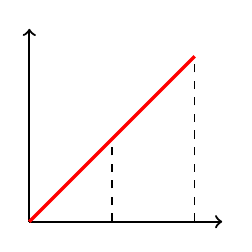
\begin{tikzpicture}[scale=0.7]
\draw[thick,->] (0,0)--(3.5,0);
\draw[thick,->] (0,0)--(0,3.5);
\draw[very thick, red] (0,0)--(3,3);
\draw[dashed] (3,0)--(3,3);
\draw[dashed] (1.5,0)--(1.5,1.5);
\end{tikzpicture}
\end{figure}

\section{Листинги}

В работах студентов кафедры <<Компьютерные технологии>> часто встречаются листинги. Листинги бывают
двух основных видов~--- исходный код и псевдокод. Первый оформляется с помощью окружения \texttt{lstlisting}
из пакета \texttt{listings}, который уже включается в стилевике и немного настроен. Пример Hello World на Java
приведен на листинге~\ref{lst1}. Пример большого листинга~--- в приложении (листинг~\ref{lstX}).

\begin{lstlisting}[float=!h,caption={Пример исходного кода на Java},label={lst1}]
public class HelloWorld {
    public static void main(String[] args) {
        System.out.println("Hello, world!");
    }
}
\end{lstlisting}

Псевдокод можно оформлять с помощью разных пакетов. В данном стилевике включается пакет \texttt{algorithmicx}.
Сам по себе он не генерирует флоатов, поэтому для них используется пакет \texttt{algorithm}.
Пример их совместного использования приведен на листинге~\ref{lst2}.

\begin{algorithm}[!h]
\caption{Пример псевдокода}\label{lst2}
\begin{algorithmic}
	\Function{IsPrime}{$N$}
		\For{$t \gets [2; \lfloor\sqrt{N}\rfloor]$}
			\If{$N \bmod t = 0$}
				\State\Return \textsc{false}
			\EndIf
		\EndFor
		\State\Return \textsc{true}
	\EndFunction
\end{algorithmic}
\end{algorithm}

Наконец, листинги из \texttt{listings} тоже можно подвешивать с помощью \texttt{algorithm},
пример на листинге~\ref{lst3}.

\begin{algorithm}[!h]
\caption{Исходный код и флоат \texttt{algorithm}}\label{lst3}
\begin{lstlisting}
public class HelloWorld {
    public static void main(String[] args) {
        System.out.println("Hello, world!");
    }
}
\end{lstlisting}
\end{algorithm}

\chapter{Проверка сквозной нумерации}

Листинг~\ref{lst4} должен иметь номер 4.

\begin{algorithm}[!h]
\caption{Исходный код и флоат \texttt{algorithm}}\label{lst4}
\begin{lstlisting}
public class HelloWorld {
    public static void main(String[] args) {
        System.out.println("Hello, world!");
    }
}
\end{lstlisting}
\end{algorithm}

Рисунок~\ref{fig2} должен иметь номер 2.

\begin{figure}[!h]
\caption{Пример рисунка}\label{fig2}
\centering
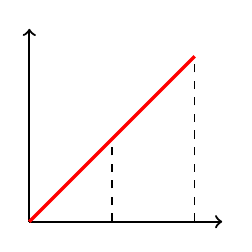
\begin{tikzpicture}[scale=0.7]
\draw[thick,->] (0,0)--(3.5,0);
\draw[thick,->] (0,0)--(0,3.5);
\draw[very thick, red] (0,0)--(3,3);
\draw[dashed] (3,0)--(3,3);
\draw[dashed] (1.5,0)--(1.5,1.5);
\end{tikzpicture}
\end{figure}

Таблица~\ref{tab3} должна иметь номер 3.

\begin{table}[!h]
\caption{Таблица умножения с помощью \texttt{tabularx} (фрагмент)}\label{tab3}
\centering
\begin{tabularx}{\textwidth}{|*{18}{>{\centering\arraybackslash}X|}}\hline
-- & 1 & 2 & 3 & 4 & 5 & 6 & 7 & 8 & 9 & 10 & 11 & 12 & 13 & 14 & 15 & 16 & 17 \\\hline
1  & 1 & 2 & 3 & 4 & 5 & 6 & 7 & 8 & 9 & 10 & 11 & 12 & 13 & 14 & 15 & 16 & 17 \\\hline
2  & 2 & 4 & 6 & 8 & 10 & 12 & 14 & 16 & 18 & 20 & 22 & 24 & 26 & 28 & 30 & 32 & 34 \\\hline
3  & 3 & 6 & 9 & 12 & 15 & 18 & 21 & 24 & 27 & 30 & 33 & 36 & 39 & 42 & 45 & 48 & 51 \\\hline
4  & 4 & 8 & 12 & 16 & 20 & 24 & 28 & 32 & 36 & 40 & 44 & 48 & 52 & 56 & 60 & 64 & 68 \\\hline
\end{tabularx}
\end{table}

\chapterconclusion

В конце каждой главы желательно делать выводы. Вывод по данной главе~--- нумерация работает корректно, ура!

%% Макрос для заключения. Совместим со старым стилевиком.
\startconclusionpage

В данном разделе размещается заключение.

\printmainbibliography

%% После этой команды chapter будет генерировать приложения, нумерованные русскими буквами.
%% \startappendices из старого стилевика будет делать то же самое
\appendix

\chapter{Пример приложения}\label{sec:app:1}

В приложениях рисунки, таблицы и другие подобные элементы нумеруются по приложениям с соответствующим префиксом. Проверим это.

Листинг~\ref{lst4:apx} должен иметь номер А.1.

\begin{algorithm}[!h]
\caption{Исходный код и флоат \texttt{algorithm}}\label{lst4:apx}
\begin{lstlisting}
public class HelloWorld {
    public static void main(String[] args) {
        System.out.println("Hello, world!");
    }
}
\end{lstlisting}
\end{algorithm}

Рисунок~\ref{fig2:apx} должен иметь номер A.1.

\begin{figure}[!h]
\caption{Пример рисунка}\label{fig2:apx}
\centering
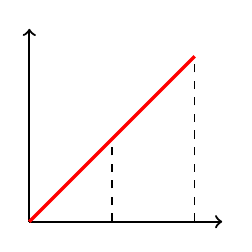
\begin{tikzpicture}[scale=0.7]
\draw[thick,->] (0,0)--(3.5,0);
\draw[thick,->] (0,0)--(0,3.5);
\draw[very thick, red] (0,0)--(3,3);
\draw[dashed] (3,0)--(3,3);
\draw[dashed] (1.5,0)--(1.5,1.5);
\end{tikzpicture}
\end{figure}

Таблица~\ref{tab3:apx} должна иметь номер A.1.

\begin{table}[!h]
\caption{Таблица умножения с помощью \texttt{tabularx} (фрагмент)}\label{tab3:apx}
\centering
\begin{tabularx}{\textwidth}{|*{18}{>{\centering\arraybackslash}X|}}\hline
-- & 1 & 2 & 3 & 4 & 5 & 6 & 7 & 8 & 9 & 10 & 11 & 12 & 13 & 14 & 15 & 16 & 17 \\\hline
1  & 1 & 2 & 3 & 4 & 5 & 6 & 7 & 8 & 9 & 10 & 11 & 12 & 13 & 14 & 15 & 16 & 17 \\\hline
2  & 2 & 4 & 6 & 8 & 10 & 12 & 14 & 16 & 18 & 20 & 22 & 24 & 26 & 28 & 30 & 32 & 34 \\\hline
3  & 3 & 6 & 9 & 12 & 15 & 18 & 21 & 24 & 27 & 30 & 33 & 36 & 39 & 42 & 45 & 48 & 51 \\\hline
4  & 4 & 8 & 12 & 16 & 20 & 24 & 28 & 32 & 36 & 40 & 44 & 48 & 52 & 56 & 60 & 64 & 68 \\\hline
\end{tabularx}
\end{table}

Заодно проверим нумерованные и ненумерованные перечисления. Ненумерованные:
\begin{itemize}
    \item пункт А;
    \item пункт Б;
    \item пункт В.
\end{itemize}

Нумерованные списки нескольких уровней:
\begin{enumerate}
    \item первый элемент;
    \item второй элемент с подэлементами:
    \begin{enumerate}
        \item первый подэлемент;
        \item второй подэлемент;
        \item третий подэлемент.
    \end{enumerate}
    \item третий элемент;
    \item четвертый элемент;
    \item пятый элемент;
    \item шестой элемент;
    \item седьмой элемент;
    \item восьмой элемент;
    \item девятый элемент;
    \item десятый элемент.
\end{enumerate}

\chapter{Еще один пример приложения с неимоверно длиннющим названием для тестирования переносов}\label{sec:app:2}

Проверим на примере таблиц, что нумерация в приложениях~--- по приложениям.
Таблица~\ref{tab3:apx2} должна иметь номер Б.1.

\begin{table}[!h]
\caption{Таблица умножения с помощью \texttt{tabularx} (фрагмент)}\label{tab3:apx2}
\centering
\begin{tabularx}{\textwidth}{|*{18}{>{\centering\arraybackslash}X|}}\hline
-- & 1 & 2 & 3 & 4 & 5 & 6 & 7 & 8 & 9 & 10 & 11 & 12 & 13 & 14 & 15 & 16 & 17 \\\hline
1  & 1 & 2 & 3 & 4 & 5 & 6 & 7 & 8 & 9 & 10 & 11 & 12 & 13 & 14 & 15 & 16 & 17 \\\hline
2  & 2 & 4 & 6 & 8 & 10 & 12 & 14 & 16 & 18 & 20 & 22 & 24 & 26 & 28 & 30 & 32 & 34 \\\hline
3  & 3 & 6 & 9 & 12 & 15 & 18 & 21 & 24 & 27 & 30 & 33 & 36 & 39 & 42 & 45 & 48 & 51 \\\hline
4  & 4 & 8 & 12 & 16 & 20 & 24 & 28 & 32 & 36 & 40 & 44 & 48 & 52 & 56 & 60 & 64 & 68 \\\hline
\end{tabularx}
\end{table}

\chapter{Пример огромного листинга}

\begin{lstlisting}[caption={Пример большого листинга},label={lstX}]
import java.util.*;

public class Example {
    static int[] restoreOutgoing(int[] g, int[] outgoing,
                                 int vertex, int mask) {
        int[] rv = new int[1 + Integer.bitCount(mask)];
        int n = g.length;
        int current = rv.length - 1;
        while (true) {
            rv[current] = vertex;
            if (current == 0) {
                if (vertex != 0) {
                    throw new AssertionError();
                }
                return rv;
            }
            mask ^= 1 << (vertex - 1);
            int prevMask = outgoing[mask] & g[vertex];
            if (prevMask == 0) {
                throw new AssertionError();
            }
            vertex = Integer.numberOfTrailingZeros(prevMask);
            --current;
        }
    }

    static int[] restoreIncoming(int[] g, int[] incoming,
                                 int vertex, int mask) {
        int[] rv = new int[1 + Integer.bitCount(mask)];
        int n = g.length;
        int current = 0;
        while (true) {
            rv[current] = vertex;
            if (current == rv.length - 1) {
                if (vertex != 0) {
                    throw new AssertionError();
                }
                return rv;
            }
            mask ^= 1 << (vertex - 1);
            int nextMask = incoming[mask] & g[vertex];
            if (nextMask == 0) {
                throw new AssertionError();
            }
            vertex = Integer.numberOfTrailingZeros(nextMask);
            ++current;
        }
    }
}
\end{lstlisting}

\end{document}
